\renewcommand{\thesubsection}{\textcolor{red}{\Roman{section}.\arabic{subsection}}}
\renewcommand{\thesubsubsection}{\textcolor{red}{\Roman{section}.\arabic{subsection}.\alph{subsubsection}}}

\setcounter{section}{0}
\setcounter{document}{0}
\sndEnTeteActDeux

\begin{center}
\begin{mdframed}[style=titr, leftmargin=60pt, rightmargin=60pt, innertopmargin=7pt, innerbottommargin=7pt, innerrightmargin=8pt, innerleftmargin=8pt]

\begin{center}
\large{\textbf{Activité documentaire : Concentration en masse et masse volumique d'une solution acqueuse.}}
\end{center}

\end{mdframed}
\end{center}

\begin{tcolorbox}[colback=orange!5!white,colframe=orange!75!black,title= Contexte de l'activité]
Consommées en excès, certaines boissons peuvent être dangereuses pour la santé à cause de leur teneur en sucre. Quelle grandeur permet d’identifier, parmi plusieurs boissons, la boisson la plus sucrée ?
\end{tcolorbox}
\begin{tcolorbox}[colback=blue!5!white,colframe=blue!75!black,title=Objectifs :]
\begin{itemize}
    \item Identifier le solvant et le(s) soluté(s) d’une solution,
    \item Déterminer la valeur de la concentration en masse d’un soluté dans une solution à partir de résultats expérimentaux,
    \item Distinguer la masse volumique d’une solution et la concentration en masse d’un soluté dans une solution.
\end{itemize}
\end{tcolorbox}

%\begin{mdframed}[style=autreexo]
%\textbf{\bsc{Consignes :}}
%\begin{itemize}
%    \item Lever la main si vous souhaitez vous déplacer,
%    \item Lever la main si vous souhaitez un indice,
%    \item Vous pouvez travailler en binôme \textbf{\underline{uniquement}} avec votre voisin de table,
 %   \item Vous pouvez rendre le travail à la fin de l'heure si vous améliorer votre note d'interrogation.
   
%\end{itemize}
%\end{mdframed}

\begin{doc}{Définitions}
\begin{tcolorbox}[colback=green!5!white,colframe=green!75!black,title=\textbf{Solution, soluté et solvant}]

\begin{wrapfigure}{r}{0.5\textwidth}
\vspace{-0.6cm}
    \centering
      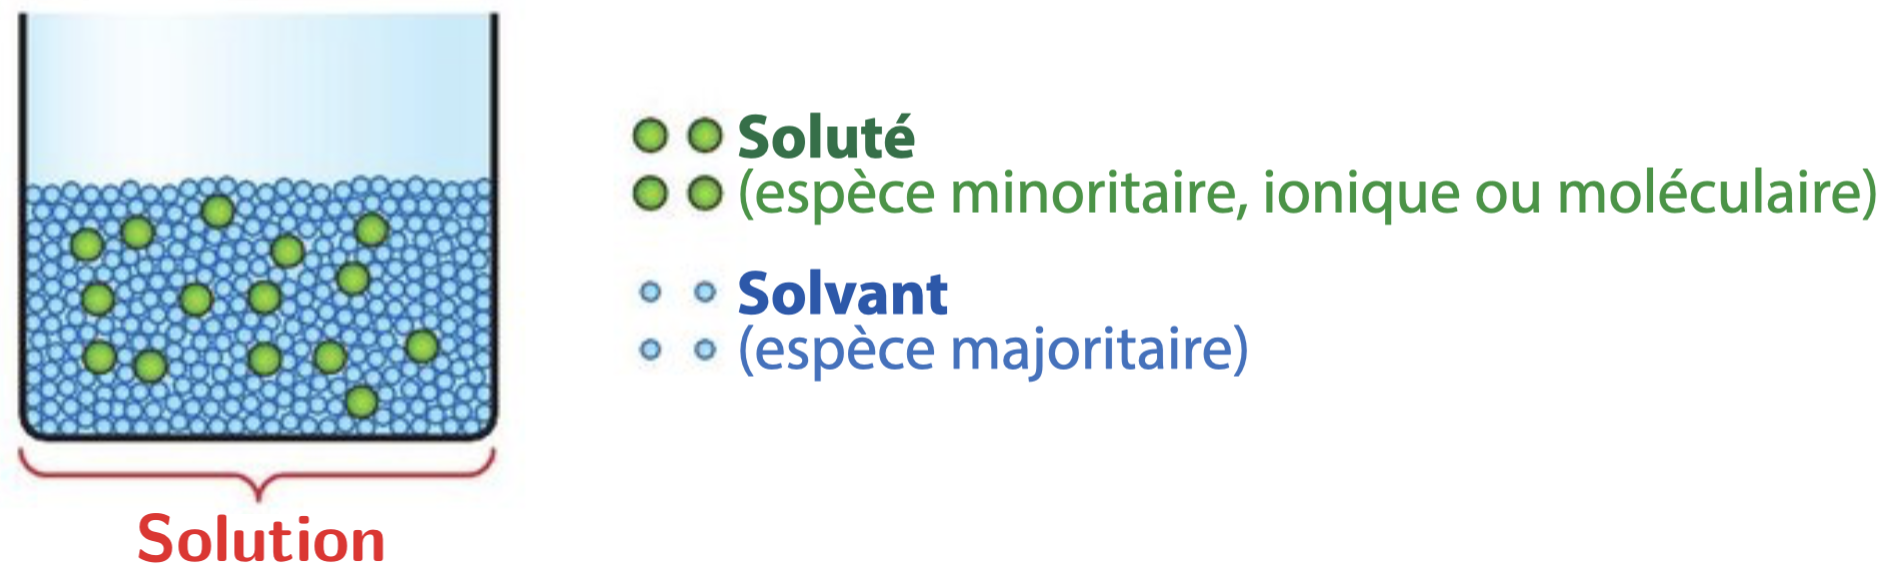
\includegraphics[width=0.5\textwidth]{Images/Activite/Chap2/Solution_solvant.png}
  \end{wrapfigure}
  Une \textbf{solution} est un mélange homogène obtenu par dissolution d’une ou plusieurs espèces chimiques appelées \textbf{solutés} dans une espèce chimique liquide appelé \textbf{solvant}.\\

  Si le solvant est l'eau, on parle de \textbf{solution acqueuse}.
\end{tcolorbox}
\begin{tcolorbox}[colback=green!5!white,colframe=green!75!black,title=\textbf{Concentration en masse}]
La \textbf{concentration en masse}, notée $C_m$,  d’un soluté dans une solution correspond à la masse de soluté dissous dans un litre de solution. Elle s’exprime par exemple en gramme par litre (g.L$^{-1}$).

\end{tcolorbox}

\end{doc}
\newpage
\begin{doc}{Données utiles sur quatre boissons sucrées}
\begin{center}
    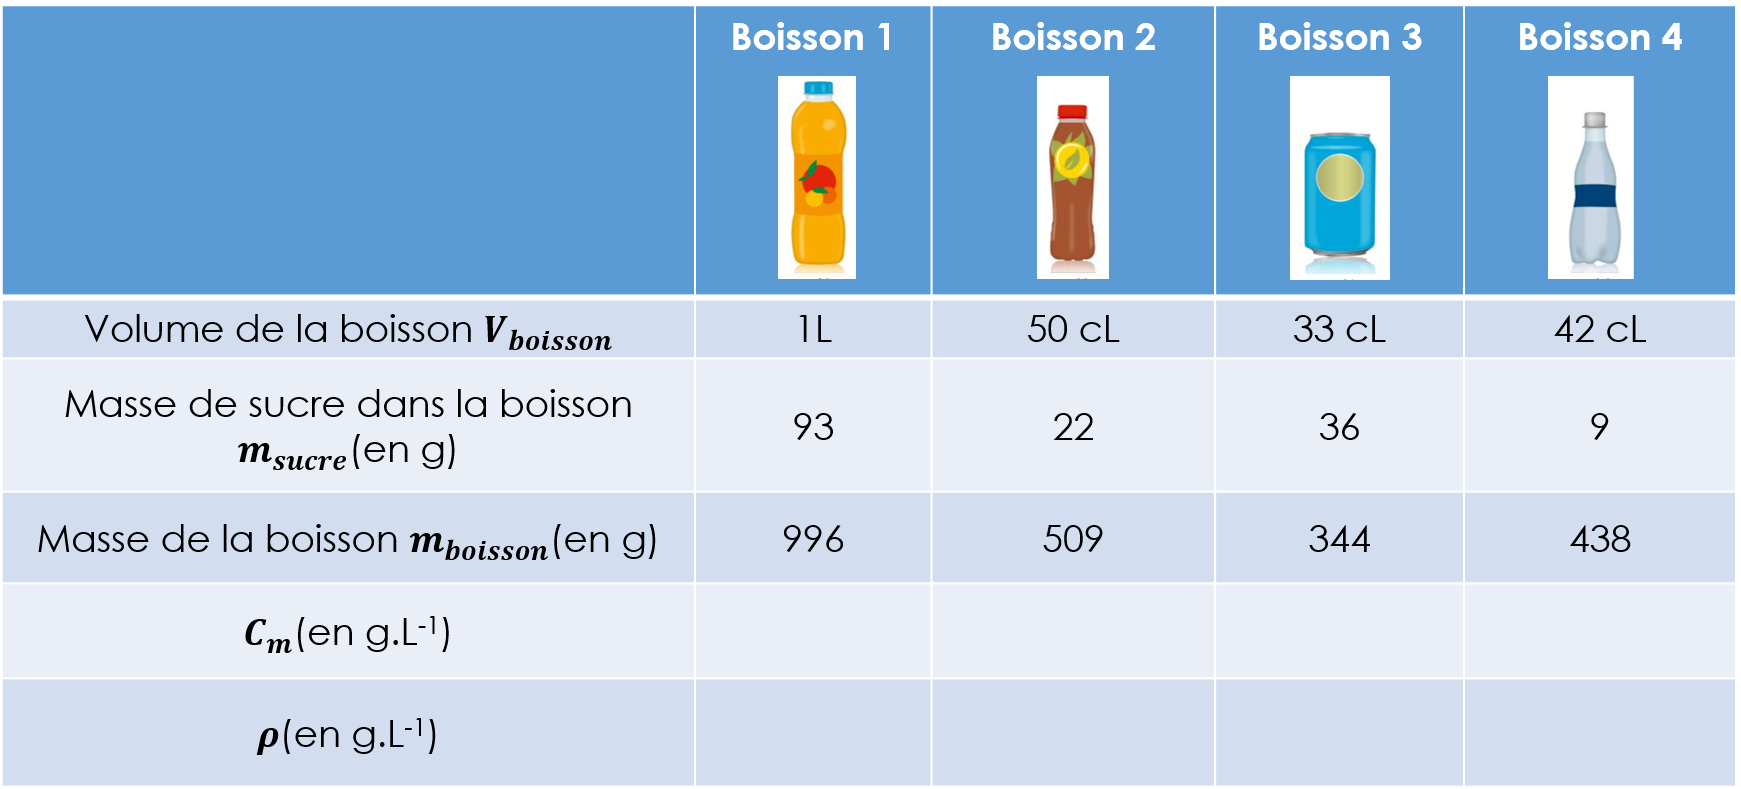
\includegraphics[scale=0.5]{Images/Activite/Chap2/Donnees.png}
\end{center}
\end{doc}

\question{Identifier le solvant et un des solutés des boissons du document 2.}{Le solvant est l'eau, les boissons sont donc des solutions acqueuses. Un soluté de la solution est le sucre car le sucre est minoritaire par rapport à l'eau.}{0}

\question{Calculer la concentration en masse de sucre $C_m$ dans chacune des boissons du document 2 en g.L$^{-1}$. Noter les résultats obtenus dans l’avant-dernière ligne du tableau de ce document.}{\begin{enumerate}
    \item Pour la boisson 1, $C_m=\frac{93}{1}=93$~g.L$^{-1}$,
    \item Pour la boisson 2, $C_m=\frac{22}{0,50}=44$~g.L$^{-1}$,
    \item Pour la boisson 3, $C_m=\frac{36}{0,33}=109$~g.L$^{-1}$,
    \item  Pour la boisson 4, $C_m=\frac{9}{0,42}=21$~g.L$^{-1}$,
\end{enumerate}}{0}

\question{Sachant qu'un morceau de sucre pèse 4,5 grammes, combien de morceaux de sucre contient la boisson la moins sucrée ? La boisson la plus sucrée ?}{La boisson la moins sucrée est la n$^\circ$4. Elle contient $\frac{9}{4,5}=2$ morceaux de sucre. La boisson la plus sucrée est la n$^\circ$3. Elle contient environ $\frac{109}{4,5}=24$ morceaux de sucre.}{0}

\question{Formuler une expression mathématique pour calculer la concentration en masse $C_m$ à partir de la masse de soluté $m_{\text{soluté}}$ et du volume $V_{solution}$ de la solution.}{En raisonnant sur les unités, on a :
\begin{equation*}
    C_m = \frac{m_{\text{soluté}}}{V_{\text{solution}}}
\end{equation*}}{0}

\question{Rappeler l’expression de la masse volumique $\rho$ d’un échantillon en précisant le nom des grandeurs utilisées.}{D'après le cours du Chapitre 1 : \begin{equation*}
    \rho = \frac{m_{boisson}}{V_{boisson}}
\end{equation*}}{0}

\question{Calculer la masse volumique $\rho$ de chacune des boissons du document 2 en g.L$^{-1}$. Noter les résultats obtenus dans la dernière ligne du tableau.}{\begin{enumerate}
    \item Pour la boisson 1, $\rho=\frac{996}{1}=996$~g.L$^{-1}$,
    \item Pour la boisson 2, $\rho=\frac{509}{0,50}=1018$~g.L$^{-1}$,
    \item Pour la boisson 3, $\rho=\frac{334}{0,33}=1012$~g.L$^{-1}$,
    \item  Pour la boisson 4, $\rho=\frac{438}{0,42}=1043$~g.L$^{-1}$.
    \end{enumerate}}{0}

\question{La concentration en masse $C_m$ d’un soluté dans une solution et la masse volumique $\rho$ d’une solution sont deux grandeurs distinctes qui peuvent être données dans la même unité (en g.L$^{-1}$ par exemple). Expliquer la différence entre la concentration en masse et la masse volumique.}{La concentration en masse permet de déterminer la masse d'un soluté contenue dans une solution. La masse volumique d'une solution est une propriété physique de la solution. Elle permet de savoir quelle sera la masse de la solution pour un volume donné}{0}